\documentclass{article}
\usepackage{tikz}

\begin{document}

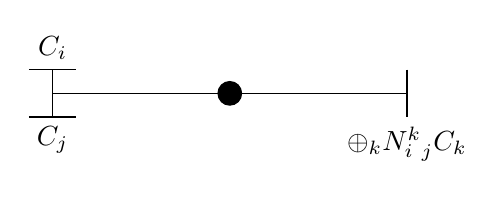
\begin{tikzpicture}[scale=1.5]
    % Draw the horizontal line with the black dot in the middle
    \draw (0,0) -- (3,0);
    \filldraw[black] (1.5,0) circle (0.1);

    % Draw the vertical lines
    \draw (0,0.2) -- (0,-0.2) node[below] {$C_j$};
    \draw (3,0.2) -- (3,-0.2) node[below] {$\oplus_k N_{i\ j}^k C_k$};

    % Draw the labels for the horizontal lines
    \draw (-0.2,0.2) -- (0.2,0.2) node[midway,above] {$C_i$};
    \draw (-0.2,-0.2) -- (0.2,-0.2) node[midway,below] {};
\end{tikzpicture}

\end{document}